% vim: set spell spelllang=en_gb ts=2 sw=2 expandtab:

\documentclass{scrreprt}
\usepackage[pdfborder={0 0 0}]{hyperref}
\usepackage{booktabs,biblatex}
\usepackage{tikz}
\bibliography{refs}
%\usepackage{graphicx,amsmath,listings,subfig}

\title{
  Beeldbewerken: Kinect project
}

\author{
  J.\ Stork, L.\ Swartsenburg,  S.\ Van Veen, B.\ Weelinck,\and J.\ Van der Woning, J.\ Zuiddam 
} % Normally, you would use \and s only, not ',' s, but this looks better.

\begin{document}

\maketitle
\tableofcontents


\chapter{Introduction}\label{ch:introduction}
    This report presents the results of a project to investigate and utilitse the
depth measurement function of Microsoft's Kinect device. For our team of six
students at the Univeristy of Amsterdam, this project concludes the
undergraduate Computer Vision course (Beeldbewerken). Like our project, this
report is in two main parts.  The first describes the key results of our
investigation into the computer vision techniques and innovations that underlie
the Kinect's depth-measurement functionality. The second part describes our
effort to build an application that utilises the Kinect to construct
three-dimensional models of relatively small objects. 



\chapter{Technical description}
\label{ch:technical}
    This chapter presents the results of our research into the technical
underpinnings of the Kinect as a sensing device. Section \ref{howitworks}
describes techniques implemented in the Kinect to produces depth maps, in terms
of standard concepts from the field of machine vision. Then, section
\ref{precision} presents measurements, estimates and published data, which
together characterise the precision of the Kinect as a measurement tool.

\section{Overview: What is a Kinect}

The Kinect device is a sensor array incorporating, most notably, a system for
depth measurement. This system relies on a technique that enables low-cost
implementations. Several founders of an Israeli technology firm, PrimeSense Ltd,
invented the technique sometime before 11 October 2005 \cite{ZALEVSKY:2007}.
Microsoft corp., in turn, began selling the Kinect-branded implementation on 10
November 2010 as an optional user interface for its consumer gaming platform,
the Xbox 360.

%describe reverse engineering, drivers, and api's in this section?
%
%common applications in this section?

\subsection{Specifications}

Table \ref{tab:specs} provides an overview of the electronic components that
comprise the Kinect's sensor array.

%nb: REF means reference to be included
%
\begin{table}[ht]
\centering
\begin{tabular}{l p{10cm}}
\toprule
Component & Description \\
\midrule

RGB Camera & Sensor ``very similar'' to Mi\-cron mt9v112 (1/6" VGA CMOS) but
``larger'' and with some di\-ffering reg\-isters. Bay\-er co\-lour pa\-ttern (RG,GB).
640x\-480 pixels, 8-bit at 30 Hz.  1280x\-1024 pixels at 10\-Hz if using Open\-NI backend
, though this is referred to as ``15Hz'' in low level pro\-tocol. UYVY co\-lour
for\-mat also possible at ``15 Hz'' framerate.\cite{FREENECT}\cite{RGBDEMO} \\

Infrared camera & Monochrome CMOS sensor (no reliable source for this). Three
options for pixel size: ``small'' (unspecified); 640x480; 1280x1024. Framerate
options are 15Hz and 30Hz, except at maximum resolution (~9Hz).\cite{FREENECT}
field of view at 57 degrees horizontal, 43 degrees vertical according to retail
description.\cite{PLAY} Range reportedly ``adjustable'' (unconfirmed source) \\ 

Depth stream & Uncompressed data stream 16 bits, though this causes device
bandwidth problems. Usable options: ``differential/RLE'' compressed 11-bit
stream; 10-bit stream; 11-bit stream (uncompressed? still to be confirmed). The
only usable pixel size is 640x480. Framerate: 30Hz. \cite{FREENECT} Depth range
1.2m to 3.5m according to retail description.\cite{PLAY} Actual range
capability: ~ 0.7m-0.6m (unconfirmed source).\\

Infrared projector & Although non-reliable internet documents refe the use of a
``laser'' to project the infrared speckle pattern, this is unconfirmed. One
patent application relating to the Kinect describes a projecting a ``pattern of
coherent radiation''.\cite{SHPUNT:2010-1} Section \ref{howitworks} provides more
detail regading the projection component. \\

Accelerometer & Kionix KXSD9 Series. Sensitivity: 819 counts per g of
acceleration. Reports device tilt relative to the
horizon.\cite{FREENECT}\cite{KIONIX}\\

Microphone & ``Multiarray'' microphone consisting of four microphone units. Each
microphone generates two streams of 32 bit signed little endian PCM samples at
16KHz. A ninth channel from the device provides a unified noise-cancelled signal
in 16-bit little endian PCM samples (16KHz).\cite{FREENECT}\\

\bottomrule
\end{tabular}
\caption{Specifications of the Kinect}
\label{tab:specs}
\end{table}


\section{Theory: How it works}
\label{howitworks}

Our assessment is that the kinect measures depth using a proprietary extension
of the standard computer vision process known as stereo triangulation. In this
section we describe the depth measurement implementation in relatively high
level terms, from the perspective of theoretical computer vision. These
descriptions are based on our interpretation of public records, including
patents and casual articles. We also refer, though to a lesser extent, to our
own experiments with the Kinect.


\subsection{Stereo triangulation}

Figure \ref{fig:triang} shows the idealised configuration of two cameras,
$c_{l}$ and $c_{r}$, set up as a stereo unit, and a point, $p$, on an object
viewed by both cameras.  In this model, we simplify: 

\begin{itemize}

    \item   the sensors as pinhole cameras;

    \item   the stereo set-up so that the image planes of the two cameras
            (represented here for convenience' sake as positioned in front of
            the focal points) are coincident;

    \item   


\end{itemize}

\begin{figure}[ht]
    \begin{center}
        \begin{tikzpicture}[scale=0.75,cap=round]

    \def\xcl{-12}
    \def\xcr{-3}
    \def\yimageplanes{1}
    \def\imageplaneshalfwidth{1.5}

    % Styles
    \tikzstyle{axes}=[]

    \begin{scope}[style=axes]
    \draw[->] (0,0) -- (-15,0) node[below] {$x$};
    \draw[->] (0,0) -- (0,10) node[above] {$z$};
    \draw[->] (0,0) -- (0.5,-0.625) node[below] {$y$};

    \end{scope}

    % point on object
    \draw [fill] (-6.5,9) circle [radius=0.025];
    \draw node [above right] at (-6.5,9) {$p$};

    % left camera
    \draw [fill] (-12,0) circle [radius=0.025];
    \draw node [below left] at (\xcl,0) {$c_{l}$};
    \draw[-] (\xcl - \imageplaneshalfwidth,\yimageplanes) -- (\xcl + \imageplaneshalfwidth, \yimageplanes);

    % right camera
    \draw [fill] (-3,0) circle [radius=0.025];
    \draw node [below right] at (\xcr,0) {$c_{r}$};
    \draw[-] (\xcr - \imageplaneshalfwidth,\yimageplanes) -- (\xcr + \imageplaneshalfwidth, \yimageplanes);

    % depth plane
    %
    % image rays
    %
    % focal length
    %
    % depth
    %
    % camera distance
    %
    % left image normal offset
    %
    % right image normal offset
    %
    % inter-offset distance

\end{tikzpicture}

        \caption{``Standard'' stereo triangulation}
        \label{fig:triang}
    \end{center}
\end{figure}


\subsection{Stereo triangulation with projected dot pattern}

% place figure for active stereo triangulation

in the kinect a corresponds to a' etc
cf slides


\subsubsection{Experiment: pattern variation over distance}

describe experiment with pictures... 


\section{Precision of the intrument}
\label{precision}


In this section we describe the Kinect's characteristics as a depth measurement
tool, and notably the precision of the measurements.


\subsection{Depth precision}

\subsubsection{Sources of error}

\subsection{Depth image resolution}

\subsubsection{Sources of error}



\chapter{Application} 
\label{ch:application}
    \lstset{ %
language=Python,                % the language of the code
basicstyle=\footnotesize,       % the size of the fonts that are used for the code
backgroundcolor=\color{white},  % choose the background color. You must add \usepackage{color}
showspaces=false,               % show spaces adding particular underscores
showstringspaces=false,         % underline spaces within strings
showtabs=false,                 % show tabs within strings adding particular underscores
frame=single,                   % adds a frame around the code
tabsize=2,                      % sets default tabsize to 2 spaces
captionpos=b,                   % sets the caption-position to bottom
breaklines=true,                % sets automatic line breaking
breakatwhitespace=false,        % sets if automatic breaks should only happen at whitespace
}


\section{Components}

What follows is a listing of application components.

\subsection{Modifications to Freenect}

Done by Jimi.

\subsection{Stereo Calibrate}

Done by Jimi.

\subsection{Creating a model}

\subsubsection{The algorithm}

%todo: with "stereo calibrate" do you mean some kinect interface module or our
%own stereo calibration step? I am assuming the latter for now...

Information derived at the stereo\texttt{stereo calibrate} stage will help with
pre-processing the Kinect image streams. We notably obtained: two intrinsic
matrices; two sets of distortion coefficients; two rotation matrices; and two
translation matrices. All these matrices can be used to undistort both images,
so that an object in the depth image is in the same place as an object in the
RGB image. We undistort the images using the \texttt{InitUndistortRectifyMap}
function from OpenCV.

With the two image streams pre-processed, the application proceeds to build the
model. The first step is to determine the ``working field''. This is done with
an A3-size sheet of white paper placed on a flat surface. The corners of the
sheet are colored (in order) green, blue, red and black.

For now, the application requires users to manually determine the orientation of
the working field. The \texttt{create\_model.py} module prompts the user to
click on the pixels in the RGB image corresponding to the coloured corners of
the A3 sheet (see figure \ref{fig:clicking}). Information displayed in the image helps the user to select the points in the correct order.

\begin{figure}[H]
\centering
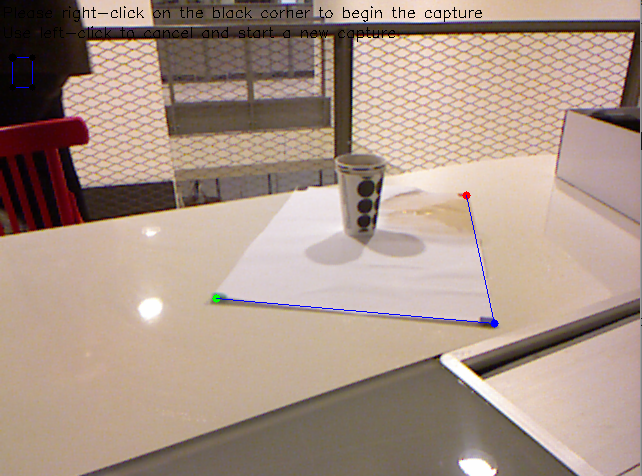
\includegraphics[scale=0.5]{images/clicking.png}
\caption{Clicking on the corners of the working field}
\label{fig:clicking}
\end{figure}

With the help of the $z$ values from the depth image, the selected points'
$(x,y,z)$ coordinates are determined. The code displayed in \ref{code:cube}
derives from this information all 8 points of a ``working cube''.\\

\begin{figure}[H]
\begin{lstlisting}
for i in xrange(4):
    cubic.append(np.array([points[i][0],points[i][1],sqrt(depth[points[i][1]][points[i][0]]]), dtype=float))
    if depth[points[i][1]][points[i][0]] > 2000:
        print "Point no. ", i, " is probably in a blind spot. Please start over."


for i in xrange(4):
    cubic = cubic + [np.cross((cubic[((i + 1) % 4)] - cubic[i]),(cubic[((i + 3) % 4)] - cubic[i]))]
    cubic[i + 4] = cubic[i + 4] / np.linalg.norm(cubic[i + 4])
    cubic[i + 4] = (cubic[i + 4] * height) + cubic[i]
\end{lstlisting}
\caption{Algorithm to create a 3 dimensional cube}
\label{code:cube}
\end{figure}

Since the working cube coordinates derived in this way are relatively
inaccurate, they are only used to overlay the cube's wireframe on the rgb and
depth images for the user's benefit. This enables the user to determine whether
they have correctly identified the working field to the application, and then to
proceed or start over as necessary.

All the ingredients to begin obtaining points for our 3d representation are now
in place:
\begin{itemize}

\item Four user-selected working field points.

\item A calibrated numpy array containing the whole RGB image as it was at the
moment of the first first click;

\item A calibrated numpy array containing the whole depth image, also from the
moment of the first click.

\end{itemize}

For each point in the image, the application needs to determine the
corresponding point in the object space. The object space was represented to the
user with the ``working cube'' wireframe. Now the application derives the axes
of the object coordinate system from the predetermined order in which the user
selected the coloured working plane corners. The following convention applies:
\begin{itemize}

\item The origin is in the corner of the cube ``above'' the green corner of the
working field.

\item The x axis runs through the origin and the working cube corner ``above'' the
working field's blue corner.

\item The y axis runs through the origin and the working field's green corner.

\item The z axis runs through the origin and the point ``above'' the working
field's black corner

\end{itemize}

The result is visualized in figure \ref{fig:axis}. \\

\begin{figure}[H]
\centering
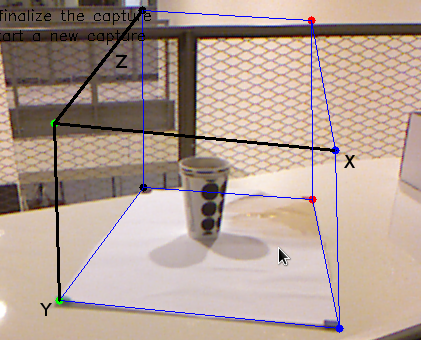
\includegraphics[scale=0.5]{images/axis.png}
\caption{Calculated cube, with axis}
\label{fig:axis}
\end{figure}

The cube's dimensions are then normalised to $100$ respectively in the $x$ and
$y$ directions, and $141$ for the $z$ direction. The last dimension is the value
of $100 * \sqrt(2)$, which in turn is the length to width ratio of an A3 sheet.
The manually selected points can now be translated to object space coordinates
as follows:
$$
\vec{green} = \left[ \begin{array}{ccc} 
0\\
100\\
0  \end{array} \right], \quad
\vec{blue} = \left[ \begin{array}{ccc} 
100\\
100\\
0  \end{array} \right], \quad
\vec{red} = \left[ \begin{array}{ccc} 
100\\
100\\
141  \end{array} \right], \quad
\vec{black} = \left[ \begin{array}{ccc} 
0\\
100\\
141  \end{array} \right].
$$
The points in object space are last information necessary to use the
\texttt{FindExtrinsic\-CameraParams2} function from OpenCV. Because the image is
undistorted during pre-processing, the identity matrix serves as the intrinsic
matrix, and \texttt{NULL} is passed as the distortion parameter. The function
returns a rotation matrix vector and a translation vector. A rotation matrix is
derived from the rotation vector using the \texttt{rodrigues2} function in
OpenCV. Then, the extrinsic matrix is derived from the translation vector. 

The resulting information can be inserted in the equation:\\
\begin{figure}
\label{eq:pipeline}
\end{figure}
\begin{equation}
s \left[ \begin{array}{ccc} 
u\\
v\\
1 \end{array} \right] = 
\left[ \begin{array}{ccc} 
f_{x} & 0 & c_{x}\\
0 & f_{y} & x_{y}\\
0 & 0 & 1 \end{array} \right] 
\left[ \begin{array}{cccc} 
r_{11} & r_{12} & r_{13} & t_{1}\\
r_{21} & r_{22} & r_{23} & t_{2}\\
r_{31} & r_{32} & r_{33} & t_{3} \end{array} \right] 
\left[ \begin{array}{ccc} 
x\\
y\\
z\\
1  \end{array} \right] 
.
\end{equation}
In this equation,
$$
\left[ \begin{array}{ccc} 
u\\
v\\
1 \end{array} \right]
$$
are the image coordinates,
$$
\left[ \begin{array}{ccc} 
x\\
y\\
z\\
1  \end{array} \right] 
$$
are the coordinates in object space,
$$
\left[ \begin{array}{ccc} 
f_{x} & 0 & c_{x}\\
0 & f_{y} & x_{y}\\
0 & 0 & 1 \end{array} \right]
$$
is the intrinsic matrix (identity) and
$$
\left[ \begin{array}{cccc} 
r_{11} & r_{12} & r_{13} & t_{1}\\
r_{21} & r_{22} & r_{23} & t_{2}\\
r_{31} & r_{32} & r_{33} & t_{3}
\end{array} \right]
$$
is the extrinsic matrix.

Now, since it has to be performed for every coordinate, calculating $s$ becomes
a costly operation. For all points in the object space, equation \ref{eq:pipeline} determines:
$$
\left[ \begin{array}{ccc} 
u s\\
v s\\
s \end{array} \right].
$$

Dividing by $s$ then yields the corresponding coordinate in the depth image.
Now, back to the four manually selected points: Every point has a corresponding
depth value in the depth image. The application selects the maximum and minimum
depth values for the four manually selected points, and stores them as boundary
values. For every point within the cube we check if the corresponding value in
the depth image is between the interpolated boundaries. If so we pass the 3d
point to the point cloud viewer. 

\subsubsection{Defects and todo}

Defects (at the time of writing):

\begin{itemize}

\item Something goes wrong in the FindExtrinsicCameraParams2, it returns NaN for the translation vector.

\item We still work with distorted images, since the stereo calibration wasn't done.

\item We don't know if the cubicle size is correct.

\item We haven't implemented anything after we needed after FindExtrinsicCameraParams2 because it doesn't work

\end{itemize}

Todo: 

\begin{itemize}

\item Undistort and rectify the images%todo

\item Find a replacement for FindExtrinsicCameraParams2%todo

\item Apply the extrinsic matrix to all object points and check if values of those points are between the depth boundaries.%todo

\item Send points to the point cloud viewer%todo

\item Color the points using the rgb image%todo

\item Auto detect the corners of our "working field"%todo

\end{itemize}

\subsection{Point Cloud Viewer}

The point cloud viewer was developed after examining various possible
bases, such as: PCL(see pointclouds.org, A very large production-class project for
anything to do with point clouds), PyGame and Visual. Visual is also know
as VPython.

For a very short period of time we tried using the mpl\_toolkit provided
by matplotlib, but as it has no support for OpenGL it isn't very suited
for rendering a large amount of points in 3D.

The PCL library was of course
very tempting, but very soon it became apparent this was way too much horse
power for our needs. What we needed was a simple interface that allowed viewing
of point clouds, rotating, moving and zooming them with mouse and keyboard
controls.

PyGame allows for very easy initialisation of OpenGL using SDL and can therefore
easily handle point clouds using most of today's graphics hardware. But it still
did not provide an easy way of controlling the camera. Rotation would require
using some sort of mathematical library implementing quaternion spherical rotation.

Enter VPython, a package attempting to implement a simple 3D programming
language on top of Python and allowing interactive terminal control of the
3D scene. VPython officially is composed of: Python (of course), IDLE the
interactive Python programming environment and the visual module. When we
discoverd the visual module used OpenGL, offers mouse orientation
controls by default, and to top it off uses NumPy for all its data manipulation
our course of action became very clear. Since the Kinect library provides its
data in NumPy arrays, after simple manipulation the point clouds can be fed into
visual with the simple command "points".

Currently the point cloud viewer does not support realtime capture, but capture
is done quickly and easily using the 'c' key.

The low-level interface includes the option for depth smoothing.

\subsection{Combining it all}

% in para below: "from files" = the matrices or the images?

The \texttt{Kinect.py} offers a user interface to the application. The file can
be executed using command line arguments to load matrices for undistoring and
rectifying the images from files. Once executed, the \texttt{Kinect.py} module
offers the user a menu. The first menu item offers a calibration process in case
this has not yet been performed.  Via the second menu choice the user can start
to build a 3d model. This opens: a point cloud viewer; an ``rgb'' screen that
displays images from the rgb camera; and a ``depth'' screen that displays depth
camera images. Whenever the user triggers an image capture, all points are sent
to the point cloud viewer. Pressing \texttt{esc} closes all windows and returns
the user to the menu.



\appendix

\chapter{Contributions} 
\label{ch:appendixA}

    This appendix presents a summary of each of the six team members' respective
contributions to this project.


\section*{Bas}
\begin{itemize}
    \item Prelimenary Kinect API testing.
    \item Point cloud viewer.
    \item OpenCV code bug fixing.
    \item Depth image to cube back projection system.
\end{itemize}

\section*{Jeroen}
\begin{enumerate}
\item eerste presentatie;
\item gewerkt aan vinden depth mapping algoritme
\end{enumerate}

\section*{Jimi}
\begin{itemize}
% Ik kan hier nog heel veel bijzetten aan tijdelijke testbestanden en zooi die ik gedaan heb, maar dat lijkt me niet echt nuttig
\item Modified Python wrappers for Freenect
\item Stereo calibration:
    \begin{itemize}
        \item theory
        \item implementation in \verb|stereo_calibrate_auto.py|
        \item tests
        \item report
    \end{itemize}
\item Alignment of images:
    \begin{itemize}
        \item theory
        \item implementation in \verb|rectify.py|
        \item tests
        \item report
    \end{itemize}
\item Getting `real' depth:
    \begin{itemize}
        \item found a good approximation
        \item implementation in \verb|rectify.py|
        \item report
    \end{itemize}
\end{itemize}

\section*{Joris}
\begin{itemize}
    \item project coordination;
    \item technical description of the Kinect (with Jeroen):
    \begin{itemize}
        \item collated and interpreted patents;
        \item collated and interpreted scholarly articles;
        \item prepared preliminary presentation;
        \item wrote technical description section of report;
    \end{itemize}
    \item edited Application section of report;
\end{itemize}

\section*{Lucas}
\begin{itemize}
\item Made up the algorithm we are using.
\item Created "create\_module.py" to implement the algorithm.
\item Created "calibrate.py" to make a calibrating framework and to do a 
straighforward single camera calibration. This was needed to better understand 
all matrices needed and to continue work on "create\_module.py".
\item Created undistort\_static.py to see the effect of the we found on some images.
\item Saved npy images so that we can work using static images (without the Kinect).
\item Created Kinect.py to combine everything.
\item Created npy\_to\_png.png to transform npy arrays to images we can open 
using a image viewer.
\item Wrote the subsections Creating a model and Combining it all in the 
application section of the report.
\item Author of the interim report.
\end{itemize}

\section*{Sander}
\begin{itemize}
    \item libfreenect and openkinect experimentation.
    \item Point cloud viewer.
    \item Depth image to cube back projection system.
\end{itemize}


\printbibliography
\end{document}
